\subsection{Wasserstein GANs (WGANs)}
\begin{frame}{}
    \LARGE GAN Variant: \\[1.5ex] \textbf{Wasserstein GANs (WGANs)}
\end{frame}

\begin{frame}[allowframebreaks]{Wasserstein GAN}
\begin{itemize}
    \item Wasserstein GAN uses the Wasserstein distance instead of the cross-entropy loss.
    \item The Wasserstein distance has a smoother gradient everywhere.
\end{itemize}
\begin{figure}
    \centering
    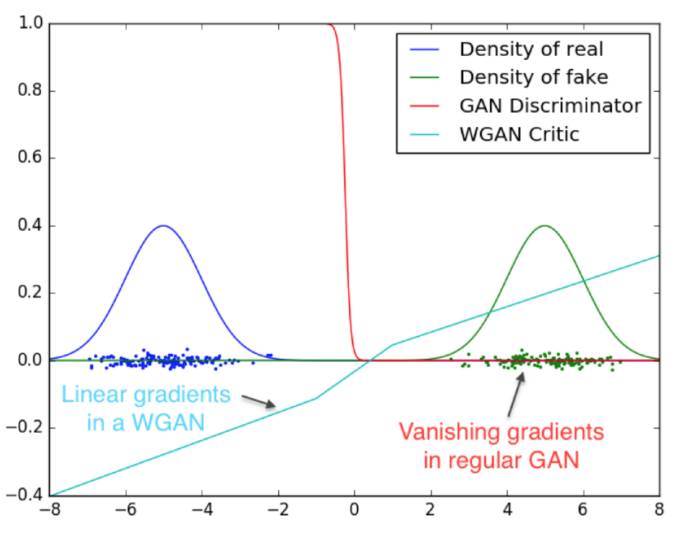
\includegraphics[height=0.6\textheight, width=\textwidth, keepaspectratio]{images/gan/wgan_1.png}
    \caption*{\scriptsize [Arjovsky, Chintala \& Bottou, ``Wasserstein GAN,'' 2017, Fig.~2]}
\end{figure}
    
\end{frame}

\begin{frame}{Wasserstein Distance}
\begin{itemize}
    \item Intuitively, it is the shovels of earth moved to make two distributions look alike.
\end{itemize}
\begin{figure}
    \centering
    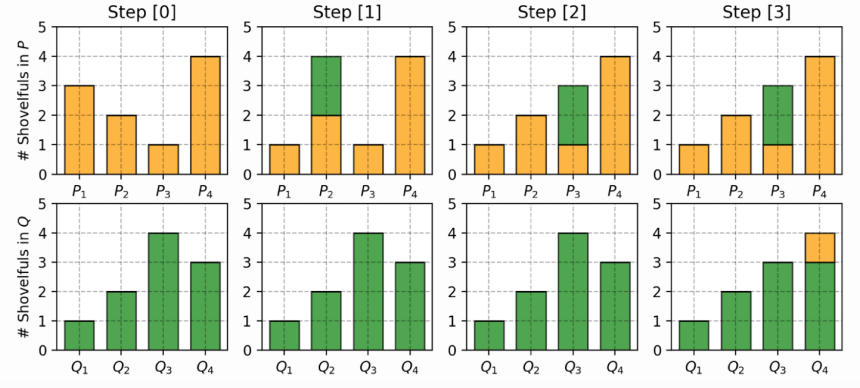
\includegraphics[height=0.6\textheight, width=\textwidth, keepaspectratio]{images/gan/wgan_2.png}
    \caption*{Step by Step plan of moving dirt between piles $P$ and $Q$ to make them match. {\scriptsize [Source: L. Weng, ``From GAN to WGAN,'' Fig.~7, \url{https://lilianweng.github.io/posts/2017-08-20-gan/}]}}
\end{figure}
\end{frame}

\begin{frame}[allowframebreaks]{WGAN}
\begin{figure}
    \centering
    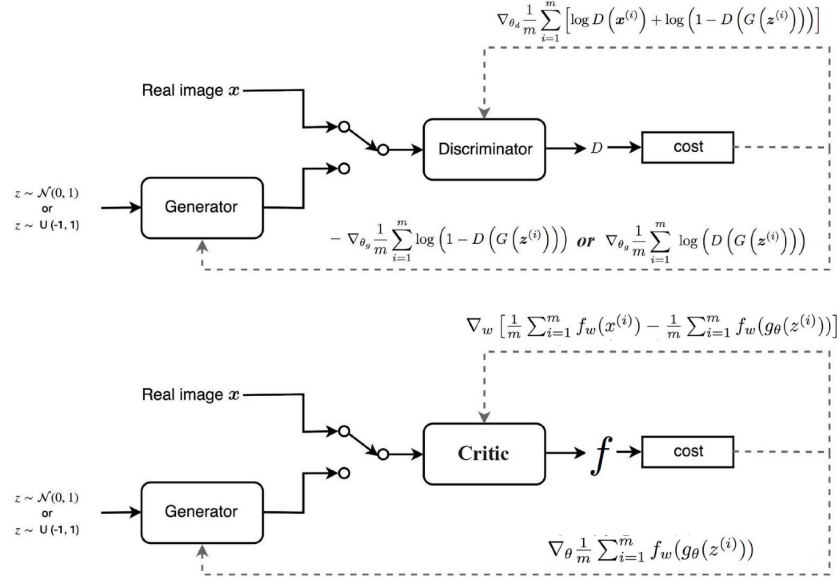
\includegraphics[height=0.82\textheight, width=\textwidth, keepaspectratio]{images/gan/wgan_3.png}
    \caption*{\scriptsize [Source: J. Hui, ``GAN: Wasserstein GAN and WGAN-GP,'' Medium, 2018]}
\end{figure}

\framebreak
\begin{figure}
    \centering
    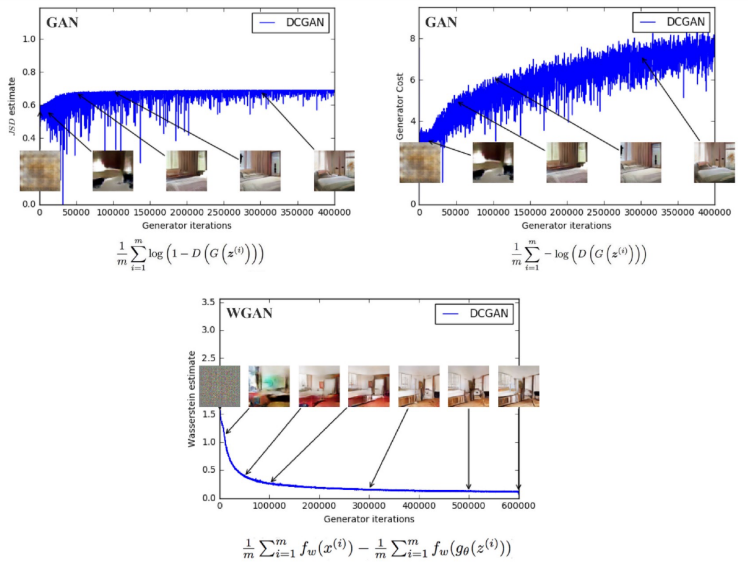
\includegraphics[height=0.78\textheight, width=\textwidth, keepaspectratio]{images/gan/wgan_4.png}
    \caption*{\scriptsize [Panels from Arjovsky, Chintala \& Bottou, ``Wasserstein GAN,'' 2017, Figs.~3, 4 and 8]}
\end{figure}

\framebreak
\begin{figure}
    \centering
    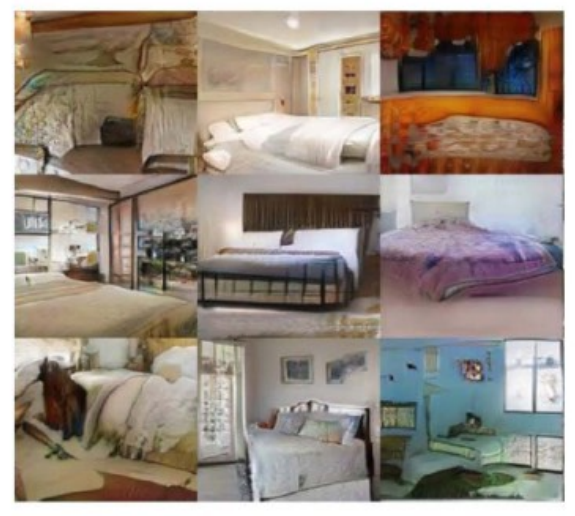
\includegraphics[height=0.8\textheight, width=\textwidth, keepaspectratio]{images/gan/wgan_5.png}
    \caption*{WGAN generation results on bedroom images. {\scriptsize [Gulrajani et al 2017, Fig.~4]}}
\end{figure}

\end{frame}

\begin{frame}[allowframebreaks]{WGAN-GP: Gradient Penalty for Lipschitzness}
\begin{figure}
    \centering
    
\includegraphics[height=0.8\textheight, width=\textwidth, keepaspectratio]{images/gan/wgan-gp/slide_84_1_img.png}
    \caption*{[Gulrajani et al 2017]}
\end{figure}

\framebreak
\begin{columns}
    \column{0.55\textwidth}
    \begin{figure}
        \centering
        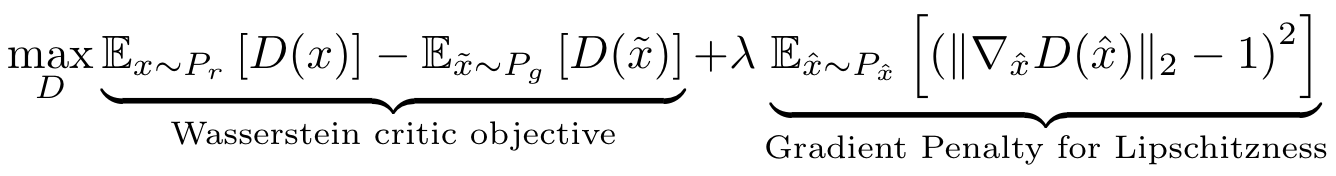
\includegraphics[height=0.72\textheight, width=\textwidth, keepaspectratio]{images/gan/wgan-gp/slide_85_3_img.png}
    \end{figure}
    \begin{figure}
        \centering
        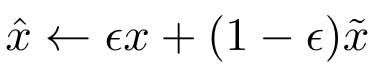
\includegraphics[height=0.08\textheight, width=\textwidth, keepaspectratio]{images/gan/wgan-gp/slide_85_4_img.png}
    \end{figure}
    \column{0.45\textwidth}
    \begin{figure}
        \centering
        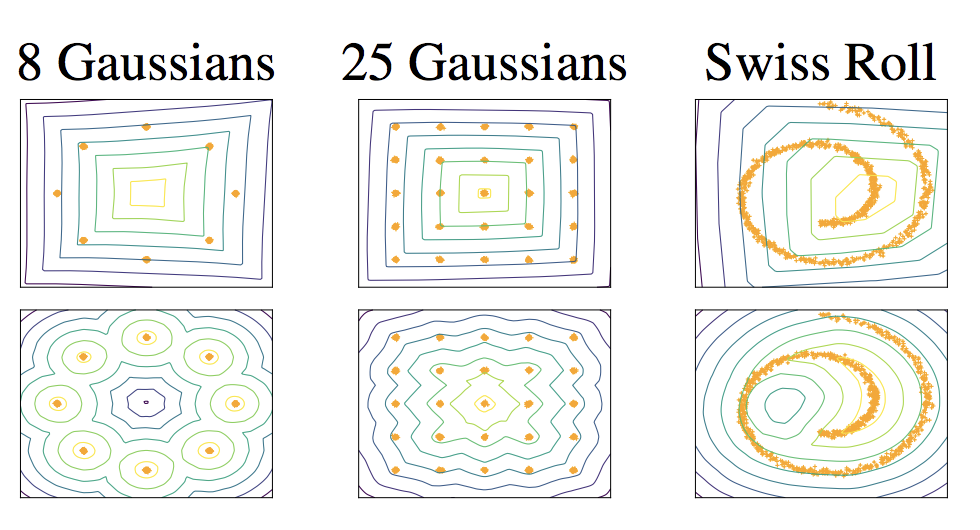
\includegraphics[height=0.38\textheight, width=\textwidth, keepaspectratio]{images/gan/wgan-gp/slide_85_2_img.png}
    \end{figure}
    \begin{figure}
        \centering
        
\includegraphics[height=0.38\textheight, width=\textwidth, keepaspectratio]{images/gan/wgan-gp/slide_85_1_img.png}
    \end{figure}
\end{columns}
{\scriptsize [Gulrajani et al 2017, Fig.~1 and Algorithm~1]}
\end{frame}

\begin{frame}[allowframebreaks]{WGAN-GP: Pseudocode}
    \begin{figure}
        \centering
        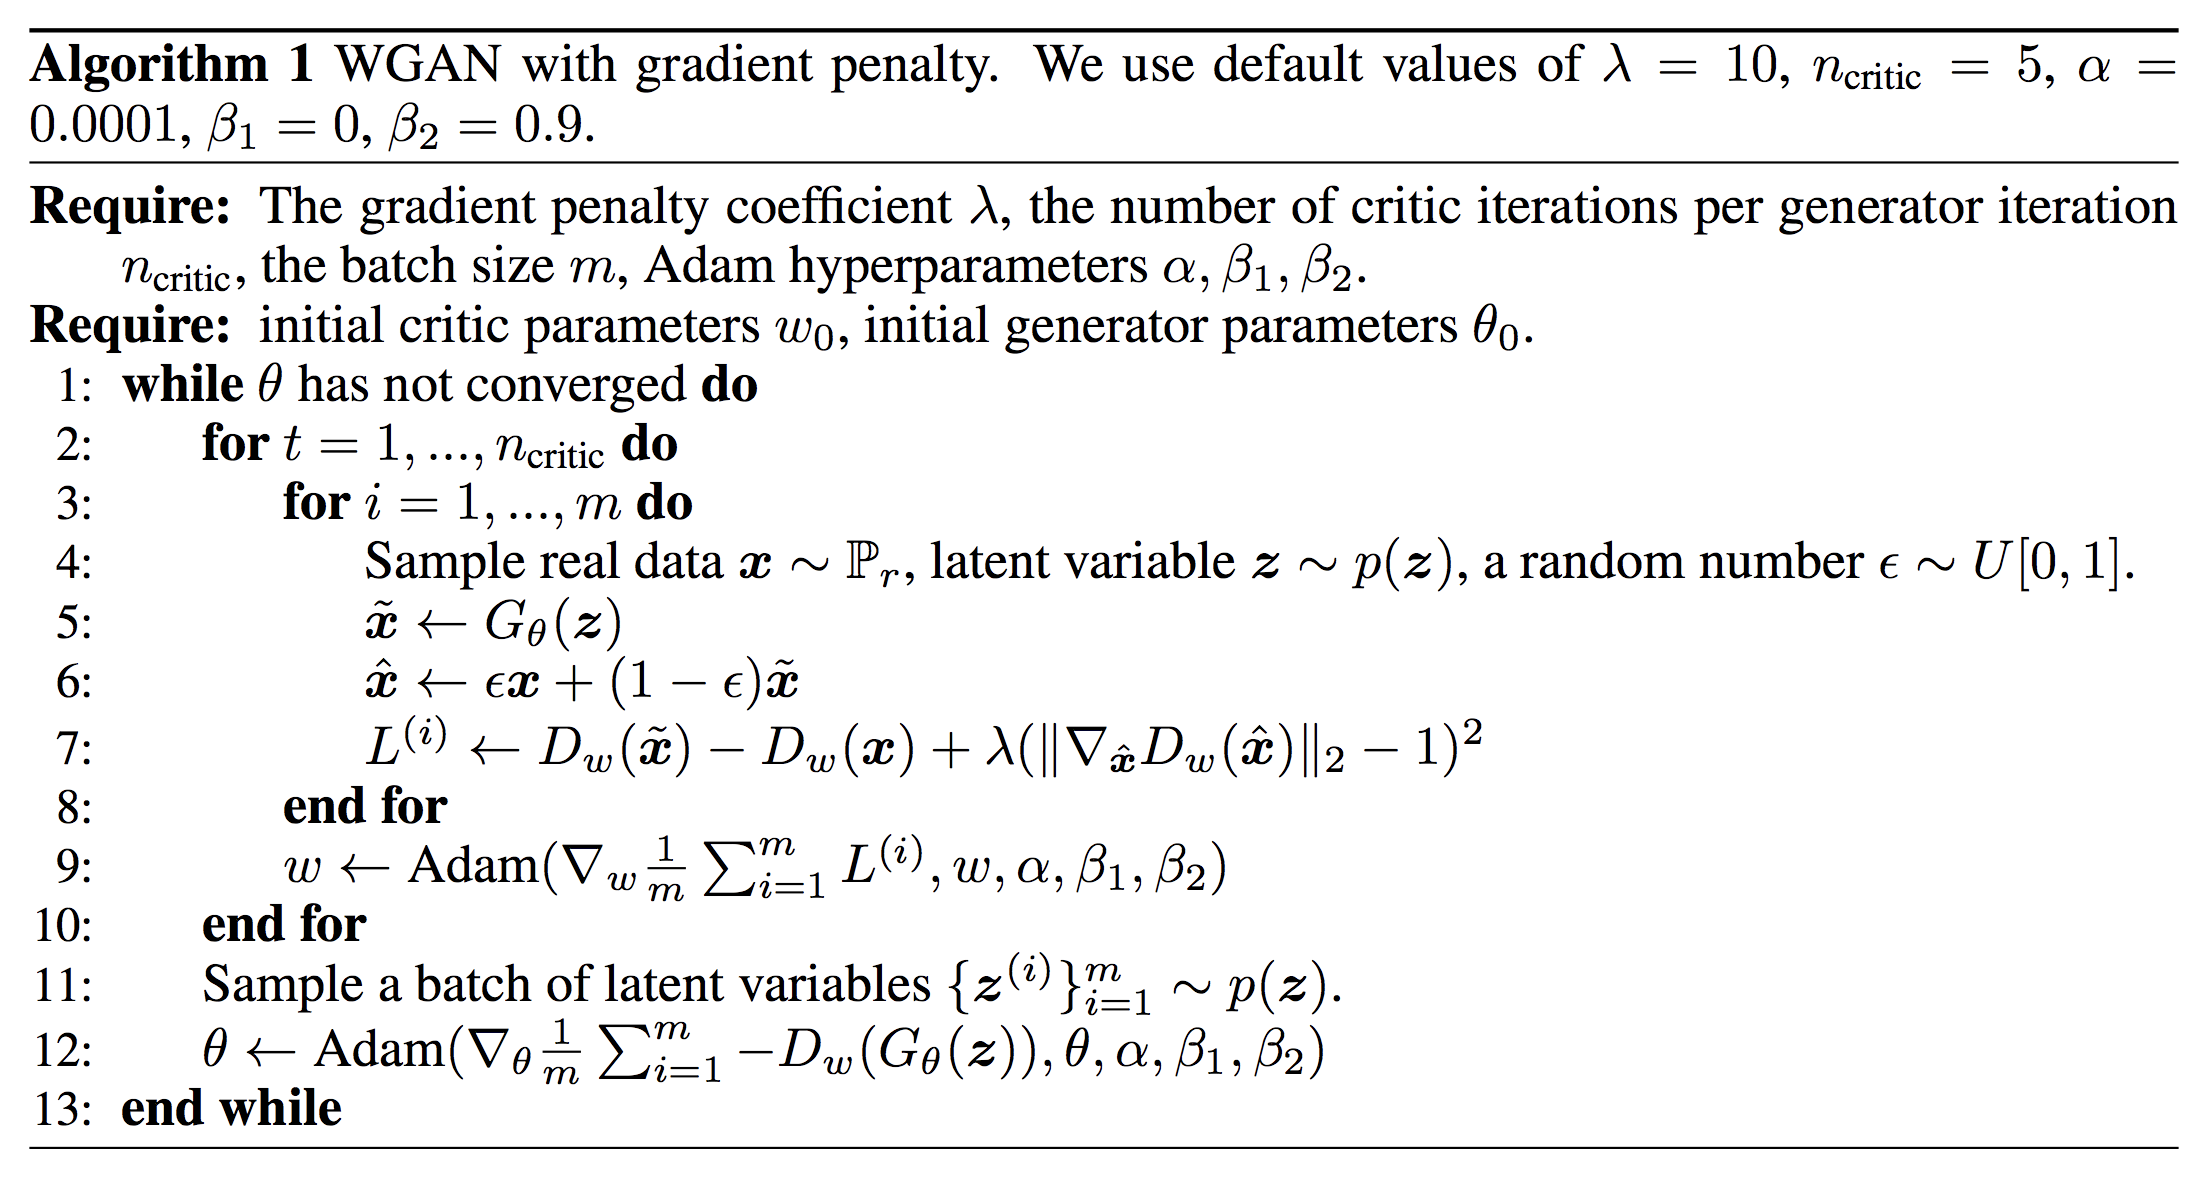
\includegraphics[height=0.8\textheight, width=1\textwidth, keepaspectratio]{images/gan/wgan-gp/slide_86_1_img.png}
        \caption*{[Gulrajani et al 2017]}
    \end{figure}
\end{frame}

\begin{frame}[allowframebreaks]{WGAN-GP: BatchNorm}
    \begin{figure}
        \centering
        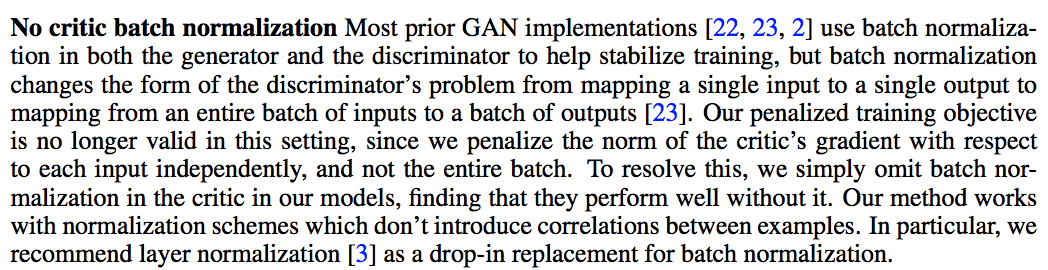
\includegraphics[height=0.8\textheight, width=1\textwidth, keepaspectratio]{images/gan/wgan-gp/slide_87_1_img.png}
        \caption*{[Gulrajani et al 2017]}
    \end{figure}
\end{frame}

\begin{frame}[allowframebreaks]{WGAN-GP: Robustness to architectures}
    \begin{figure}
        \centering
        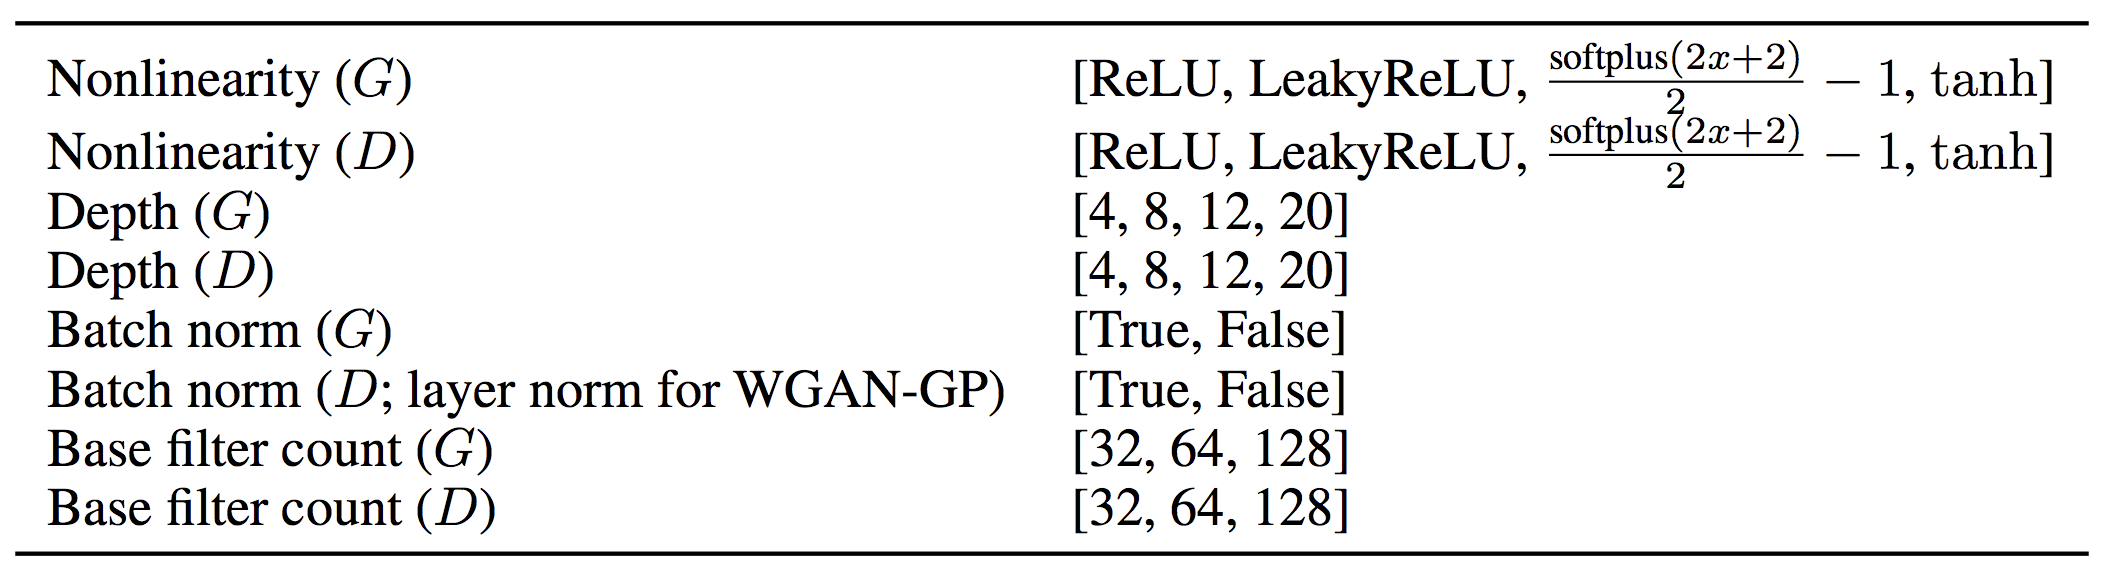
\includegraphics[height=0.7\textheight, width=.8\textwidth, keepaspectratio]{images/gan/wgan-gp/slide_88_1_img.png}
    \end{figure}
    \begin{figure}
        \centering
        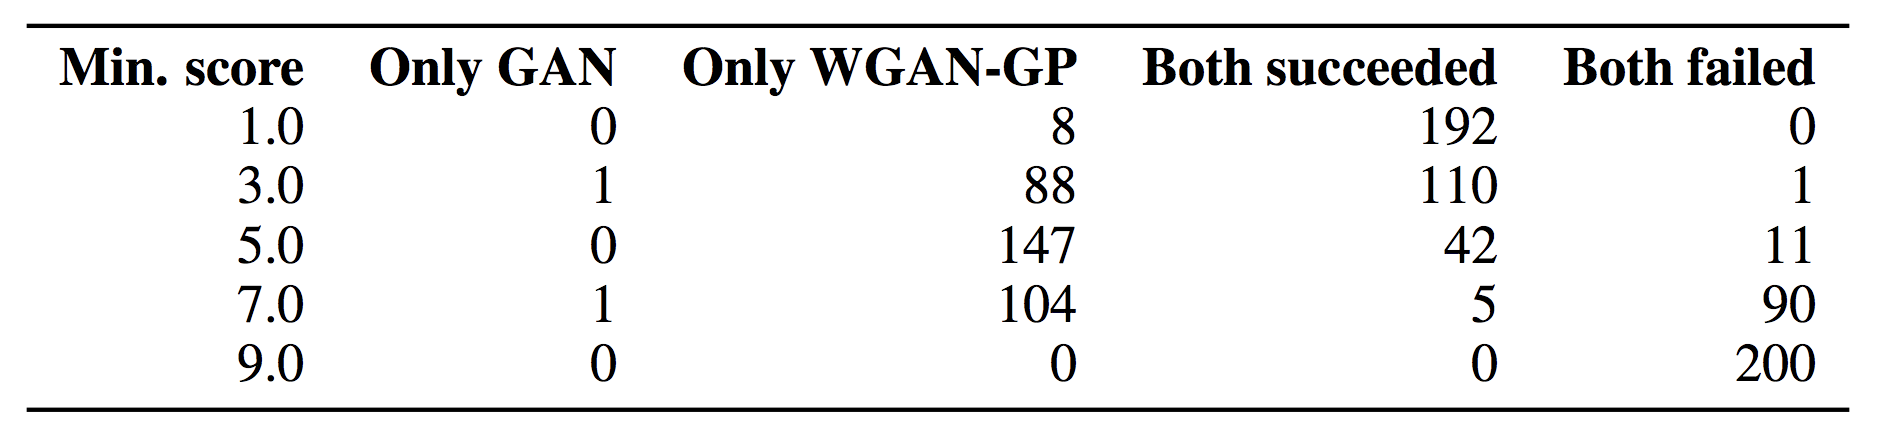
\includegraphics[height=0.7\textheight, width=.8\textwidth, keepaspectratio]{images/gan/wgan-gp/slide_88_2_img.png}
        \caption*{[Gulrajani et al 2017]}
    \end{figure}

    \framebreak

    \begin{figure}
        \centering
        
\includegraphics[height=0.7\textheight, width=.8\textwidth, keepaspectratio]{images/gan/wgan-gp/slide_89_1_img.png}
        \caption*{[Gulrajani et al 2017]}
    \end{figure}
\end{frame}


\begin{frame}[allowframebreaks]{WGAN-GP: High quality samples}
    \begin{figure}
        \centering
        
\includegraphics[height=0.8\textheight, width=1\textwidth, keepaspectratio]{images/gan/wgan-gp/slide_90_1_img.png}
        \caption*{[Gulrajani et al 2017]}
    \end{figure}

    \framebreak

    \begin{figure}
        \centering
        
\includegraphics[height=0.8\textheight, width=1\textwidth, keepaspectratio]{images/gan/wgan-gp/slide_91_1_img.png}
        \caption*{[Gulrajani et al 2017]}
    \end{figure}
\end{frame}